\documentclass[border=0.2cm]{standalone}
\usepackage{tikz}
\usetikzlibrary{calc}
\usetikzlibrary{intersections} % Necessário para achar pontos de cruzamento

\begin{document}
\pagestyle{empty}

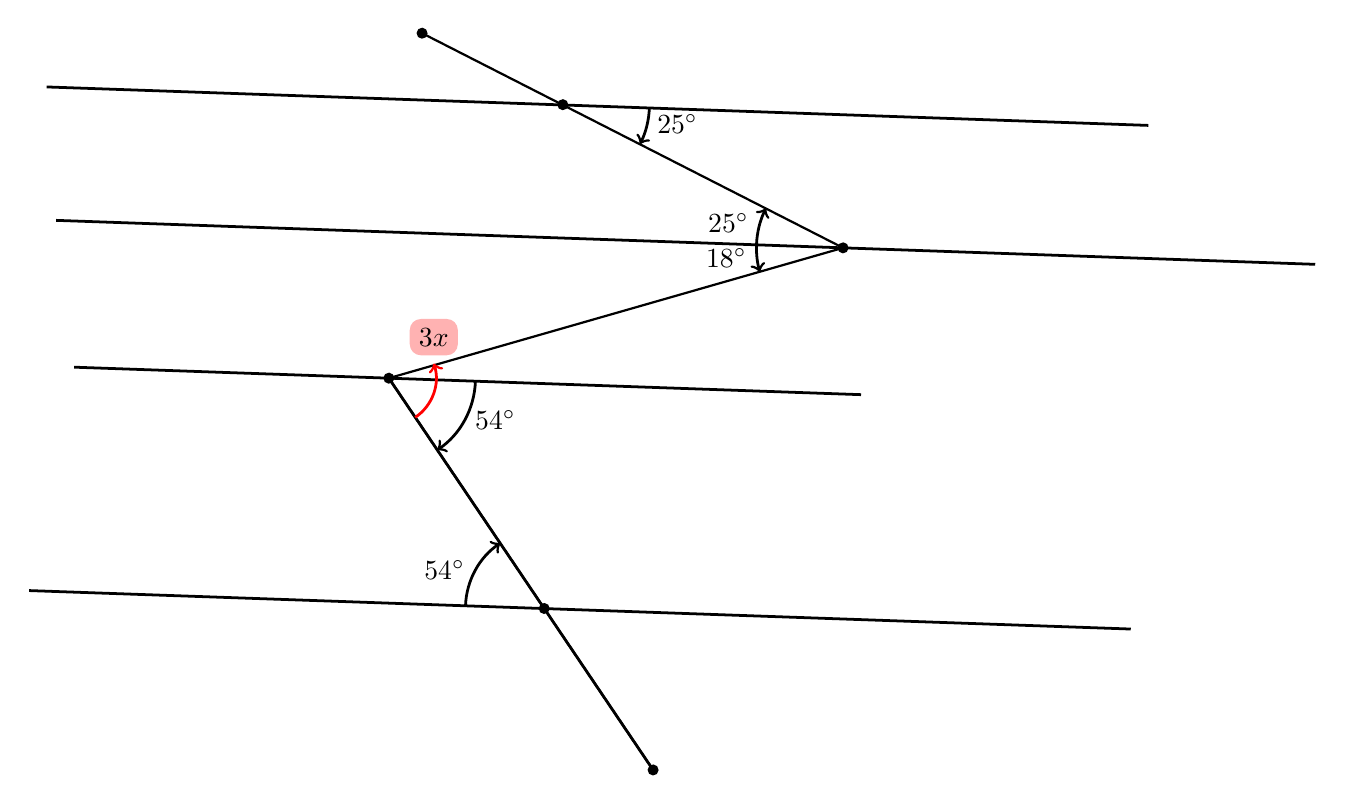
\begin{tikzpicture}[scale=2,line width=1pt,rotate=-2]
  %\draw[help lines,black!30] (-5.5,-5.5) grid (5.5,5.5);
  %\draw[thick,->] (0,-5) -- (0,5) node[left]  {y};
  %\draw[thick,->] (-5,0) -- (5,0) node[below] {x};
  %\foreach \x in {-4,-3,-2,-1,1,2,3,4} \node[left,color=red] at (0,\x) {\x} node[below,color=red] %at (\x,0) {\x};
  %\node[below right,color=red] at (0,0) {0}; 
 
  %\foreach \x in {-2,...,2} {\draw[thick] (-4,\x) -- (4,\x);}

  
    \coordinate (A) at (0,0);
    \coordinate (B) at (180-54:3cm);
    \coordinate (C) at ($(B)+(18:3cm)$);
    \coordinate (D) at ($(C)+(180-25:3cm)$);
    
    \draw[thick] (A) -- (B) -- (C) -- (D);
    

    \draw (B) -- +(3,0) -- +(-2,0);
    \draw (C) -- +(3,0) -- +(-5,0);

    \draw[name path=lineD] (-4,4.2) -- +(7,0);
    \draw[name path=lineA] (-4,1) -- +(7,0);

    \fill (A) circle (1pt); % node[above left] {A};
    \fill (B) circle (1pt); % node[above left] {B};
    \fill (C) circle (1pt); % node[above left] {C};
    \fill (D) circle (1pt); % node[above left] {D};

    \draw[name path=AB] (A) -- (B);
    \path[name path=CD] (C) -- (D);
    
    \path[name intersections={of=lineD and CD}] coordinate (interA)  at (intersection-1);
    \path[name intersections={of=lineA and AB}] coordinate (interB)  at (intersection-1);
 
    \fill (interA) circle (1pt); % node[above right] {interA};
    \fill (interB) circle (1pt); % node[above right] {interB};


% Arco 1 vermelho (B) (interB)
    \draw[<-] ($(interB)+(180-54:5mm)$)  arc (180-54:180:5mm) node[midway,left] {$54^\circ$};
    \draw[->] ($(B)+(0:5.5mm)$)  arc (0:-54:5.5mm) node[midway,right] {$54^\circ$};
    %\draw[black!50,->] ($(interB)+(0:7mm)$)  arc (0:360:7mm);

% Arco 2 azul (B) (C)
   \draw[red,->] ($(B)+(-54:3mm)$)  arc (-54:20:3mm) node[above,yshift=.5pt,fill=red!30,text=black,rounded corners,yshift=2pt] {$3x$};
   \draw[->] ($(C)+(180:5.5mm)$)  arc (180:180+18:5.5mm) node[midway,left] {$18^\circ$};

% Arco 2 azul (C) (interA)
   \draw[->] ($(C)+(180:5.5mm)$)  arc (180:180-25:5.5mm) node[midway,left,yshift=1pt] {$25^\circ$};
   \draw[->] ($(interA)+(0:5.5mm)$)  arc (0:-25:5.5mm) node[midway,right,yshift=1pt] {$25^\circ$};

\end{tikzpicture}

\end{document}